%% Include the picture as follows: \
% \begingroup
% \tikzset{every picture/.style={scale=1,radius=0.05,line width=0.4}}%
% \input{tikz/[filename].tex}%
% \endgroup
%
%% Want to add a label? Use node[<position>]{label},
%% where <position> is one of: below / above / left / right
% \fill (0,0) circle node[below]{$p_1$};
%% Want to give the point a different color?
% \fill[red] (0,0) circle;
%
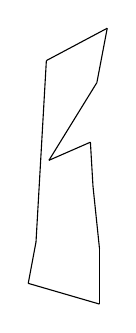
\begin{tikzpicture}
\draw (7.9572,5.0954) -- (8.4836,5.3257);
\draw (7.6941,3.5329) -- (8.5987,3.2697);
\draw (8.5987,3.9770) -- (8.5987,3.2697);
\draw (8.5164,4.7664) -- (8.5987,3.9770);
\draw (8.5658,6.0822) -- (7.9572,5.0954);
\draw (7.7928,4.0592) -- (7.6941,3.5329);
\draw (7.9243,6.3618) -- (7.7928,4.0592);
\draw (8.4836,5.3257) -- (8.5164,4.7664);
\draw (8.6974,6.7730) -- (8.5658,6.0822);
\draw (7.9243,6.3618) -- (8.6974,6.7730);
\fill (7.9243,6.3618) circle;
\fill (7.9572,5.0954) circle;
\fill (7.7928,4.0592) circle;
\fill (7.6941,3.5329) circle;
\fill (8.6974,6.7730) circle;
\fill (8.5658,6.0822) circle;
\fill (8.4836,5.3257) circle;
\fill (8.5164,4.7664) circle;
\fill (8.5987,3.9770) circle;
\fill (8.5987,3.2697) circle;
\end{tikzpicture}
